\lecture{7}{Mo 03 Mai 2021 10:17}{Bedingte Wahrscheinlichkeit}
\section{Bedingte Wahrscheinlichkeit und Unabhängigkeit}
\subsection{Bedingte Wahrscheinlichkeit}
\begin{example}
    Es werden statistische Daten über Kleinkinder gemessen: Wann sie krabbeln und wann sie laufen. Betrachten wir die Ereignisse
    \[
        A = \left \{\text{Kind läuft vor dem 10. Monat}\right\}  \qquad B = \left \{\text{Kind krabbelt vor dem 6. Monat}\right\} 
    .\] 
    Aus den Daten geht hervor, dass $\mathbb{P}(A) = 25 \%$ und $\mathbb{P}(B) = 20\%$.
    \begin{question}
        Sei ein Kind, das mit 6 Monaten krabbelt, gegeben. Wie hoch ist die Wahrscheinlichkeit, dass es mit 10 Monaten schon läuft?
    \end{question}
    Wir brauchen mehr Information als die obige, um die Frage beantworten zu können! Wir gehen also davon aus, dass wir sogar folgende Daten zur Verfügung haben: \\
    \begin{minipage}{\textwidth}
        \begin{minipage}{0.5\textwidth}
            \centering
    \begin{tabular}{c|c|c}
        $\cap$ & $A$ & $A^{c}$ \\
        \hline
        $B$ & \emphasize{0,15} & \emphasize{0,05} \\
        $B^{c}$ & \emphasize{0,10} & \emphasize{0,70}
    \end{tabular}
        \end{minipage}
        \begin{minipage}{0.5\textwidth}
            \centering
            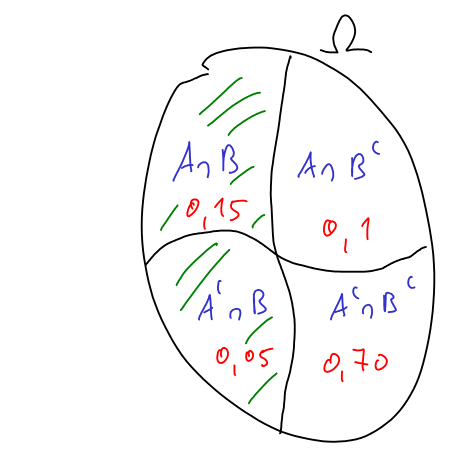
\includegraphics[scale=0.2]{figures/Bedingte Wahrscheinlichkeit.png}
        \end{minipage}
    \end{minipage}
    \\
    Wir wissen, dass $B$ eintritt, also befinden wir uns bereits im Zustandsraum  $\Omega_B := \left \{w\in \Omega \mid  w\in B\right\} $. Ziel ist es also, eine neue Massenfunktion $\mathbb{P}(\cdot |B)$ (auf $\Omega$) zu definieren, die die Information '$\omega\in B$' berücksichtigt. Insbesondere muss also gelten:
    \[
        \mathbb{P}(\omega | B) = 0 \qquad \forall\; \omega\in \Omega_B^{c}
    .\] 
    Zudem wollen wir, dass die Information '$\omega \in B$' dieselbe ist für alle $w\in \Omega_B$, d.h.
    \[
        p(\omega|B) = \subset \cdot p(\omega) \qquad \forall \; \omega\in \Omega_B
    .\] 
    wobei $p(\omega)$ die Massenfunktion von $\mathbb{P}$ ist. Wegen Normierung ergibt sich also bereits
    \[
        1 = \sum_{\omega\in \Omega} \mathbb{P}(\omega|B) = o\cdot \sum_{\omega\in \Omega_B} p(\omega) \quad \iff  \quad c = \frac{1}{\mathbb{P}(B)}
    .\] 
    Also ergibt sich, dass 
    \[
        p(\omega\mid B) = \begin{cases}
            \frac{p(\omega)}{\mathbb{P}(B)} & \text{falls } \omega\in B \\
            0 & \text{sonst}
        \end{cases}
    .\] 
    Wir können das ganze so darstellen: \\
    \begin{minipage}[t]{\textwidth}
        \centering
        \vspace{-2ex}
    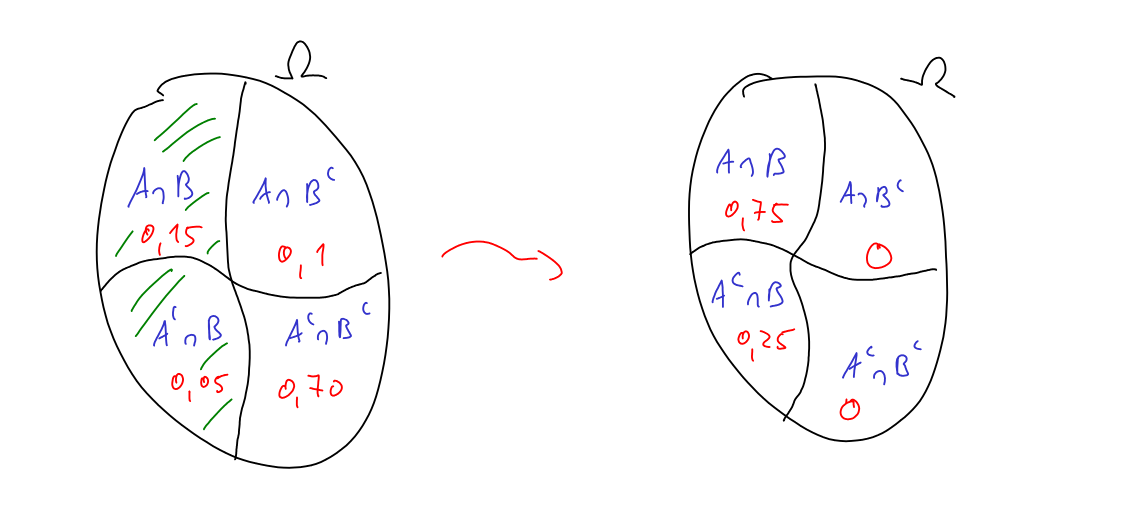
\includegraphics[scale=0.2]{figures/Bedingte Wahrscheinlichkeit II.png}
    \captionof{figure}{Änderung des Zustandsraums bei bedingten Wahrscheinlichkeiten}
    \vspace{2ex}
    \end{minipage}
    Wir erhalten also:
    \begin{answer}
        Ein Kind, das mit 6 Monaten krabbelt, wird mit einer Wahrscheinlichkeit von $75\%$ mit 10 Monaten laufen können.
    \end{answer}
\end{example}
\todo{Besser Skizzen machen}
\begin{definition}[Bedingte Wahrscheinlichkeit]\label{def:bedingte-wahrscheinlichkeit}
    Sei $(\Omega, \mathcal{F}, \mathbb{P})$ ein Wahrscheinlichkeitsraum. Seien $A,B\in \mathcal{F}$ Ereigniss mit $\mathbb{P}(B) \neq  0$. Dann definieren wir
    \[
        \mathbb{P}(A \mid B) := \frac{\mathbb{P}(A\cap B)}{\mathbb{P}(B)}
    .\] 
    und nennen dise die \vocab[Wahrscheinlichkeit!bedingte]{bedingte Wahrscheinlichkeit von $A$ gegeben  $B$}. 
\end{definition}
\begin{remark}
       Die Abbildung
               \begin{equation*}
                   \mathbb{P}(\cdot \mid B): \left| \begin{array}{c c l} 
               \mathcal{F} & \longrightarrow & \R_+ \\
               A & \longmapsto &  \mathbb{P}(A\mid B)
               \end{array} \right.
           \end{equation*}
           ist eine Wahrscheinlichkeitsverteilung auf $(\Omega,\mathcal{F})$, die wir auch die \vocab[Wahrscheinlichkeitsverteilung!bedingte]{bedingte Wahrscheinlichkeitsverteilung gegeben $B$} nennen.
\end{remark}
\begin{definition}[Bedingter Erwartungswert]\label{def:bedingter-erwartungswert}
    Sei $X:\Omega\to \mathcal{S}\subset \R$ eine (diskrete) Zufallsvariable mit Verteilung $\mathbb{P}(\cdot \mid B)$. Dann hat $X$ den Erwartungswert
    \[
        \sum_{s\in \mathcal{S}} s\cdot \mathbb{P}(X = s | B) =: \mathbb{E}(X\mid B)
    .\] 
    Dieser heißt \vocab[Erwartungswert!bedingter]{bedingter Erwartungswert von $X$ gegeben  $B$}. 
\end{definition}
\begin{example}
    Wir werfen eine faire Münze $N$ mal, dabei beobachten wir $n$ mal das Ergebnis 'Zahl'.
     \begin{question}
        Was ist die Wahrscheinlichkeit, dass bei den ersten $m$ Würfen immer 'Zahl' gefallen ist?
    \end{question}
    Ohne Weitere Informationen (dass insgesamt $n$ mal Zahl gefallen ist) würden wir hier $\mathbb{P} \equiv \frac{1}{2^m}$ erhalten. \\
    Betrachte nun den Zustandsraum
    \[
        \Omega = \left \{\omega = (x_1,\ldots,x_N)\mid x_i \in \left \{0,1\right\},1\leq i\leq N \right\} 
    .\] 
    wobei
    \[
    x_k := \begin{cases}
        1 & \text{falls $k$-ter Wurf ist 'Zahl'} \\
        0 & \text{falls $k$-ter Wurf ist 'Kopf'}
    \end{cases}
    .\] 
    und versehe ihn mit $\mathcal{F} = \mathcal{P}(\Omega)$ sowie $\mathbb{P}$ als Gleichverteilung auf $\Omega$. Mit $X_k(\omega) := x_k$ interessieren wir uns also für
    \[
        \mathbb{P}\left(X_1=X_2=\ldots=X_m =1 \mid  \sum_{k=1}^N X_k  =n\right)
    .\]
    Nach Definition ist dies
    \[
        \begin{split}
        &= \frac{\mathbb{P}\left(\left(X_1=\ldots=X_m = 1\right) \cap  \left(\sum\limits_{k=m+1}^N X_k = n-m\right)\right)}{\mathbb{P}\left(\sum\limits_{k=1}^N X_k = n\right)} \\
        &= \frac{\frac{1}{2^N} \binom{N-m}{n-m}}{\frac{1}{2^N}\binom{N}{n}} \\
        &= \frac{(N-m)!}{(n-m)!(N-n)!} \cdot  \frac{(N-n)! n!}{N!} \\
        &= \frac{(N-m)! n!}{N! (n-m)!}
        \end{split}
    .\] 
\end{example}
\begin{notation}
    Zur Vereinfachung der Notation schreiben wir oft
    \[
    \mathbb{P}(X_1=X_2=a) = \mathbb{P}(\left \{\omega\in \Omega \mid  X_1(\omega) = a\right\} \cap \left\{ \omega\in \Omega \mid X_2(\omega) =a\right\} )
    .\] 
    sowie
    \[
    \mathbb{P}(X_1=a, X_2=b) = \mathbb{P}(\left \{\omega\in \Omega \mid  X_1(\omega) = a \right\} \cap \left\{\omega\in \Omega\mid X_2(\omega)  =b\right\} )
    .\] 
\end{notation}
Wir haben gerade aus einer Wahrscheinlichkeitsverteilung $\mathbb{P}$ die Verteilung $\mathbb{P}(\cdot \mid B)$ gewonnen. Das ganze geht auch umgekehrt:
\begin{theorem}\label{thm:zerlegung-in-ereignisse-ergibt-aufaddieren-bedingter-wahrscheinlichkeiten}
    Sei $\Omega = \bigcup_{k\in I} H_k$ eine \emphasize{disjunkte} Zerlegung von $\Omega$ in (abzählbar viele) Ereignisse $H_k, k\in I$, wobei $\mathbb{P}(H_k) \neq 0$. Dann ist $\forall A\in \mathcal{F}$:
    \[
        \mathbb{P}(A) = \sum_{k\in I} \mathbb{P}(A \mid H_k) \cdot \mathbb{P}(H_k)
    .\] 
\end{theorem}
\begin{proof}
    $\forall A\in \mathcal{F}$ ist
    \[
        A= A \cap  \bigcup_{k\in I} H_k = \bigsqcup_{k\in I} (A\cap H_k) 
    .\] 
    eine disjunkte Vereinigung. Also folgt aus $\sigma$-Additivität, dass
    \begin{equation*}
        \begin{split}
            \mathbb{P}(A) &= \sum_{k\in I} \mathbb{P}(A\cap H_k) \\
                          &= \sum_{\substack{ k\in I\\ \mathbb{P}(H_k)\neq 0}} \mathbb{P}(A\cap H_k) \\
                          &=\sum_{\substack{ k\in I \\ \mathbb{P}(H_k)}\neq 0} \mathbb{P}(A\mid H_k) \cdot  \mathbb{P}(H_k)
        \end{split}
    \end{equation*}
\end{proof}
\begin{example}
    Eine Urne $A$ enthält {\color{red} 2 rote} und {\color{blue} 3 blaue} Kugeln. In Urne  $B$ liegen umgekehrt {\color{red} 3 rote} und nur {\color{blue} 2 blaue} Kugeln. Wir gehen davon aus, dass die Urnen immer gut gemischt sind. Nun machen wir Folgendes:
    \begin{enumerate}[label=\protect\circled{\arabic*}]
        \item Wir ziehen eine Kugel $K_1$ aus $A$ und legen sie in  $B$
        \item Wir ziehen eine Kugel  $K_2$ aus $B$ und lg
    \end{enumerate}
    \begin{question}
    Was ist die Wahrscheinlichkeit, dass $K_2$ {\color{red} rot} ist?
    \end{question}
Wir erhalten nun
\[
    \begin{split}
        \mathbb{P}(K_2 \text{ ist rot}) &= \mathbb{P}(K_2 \text{ rot} \mid  K_1 \text{ rot})\cdot \mathbb{P}(K_1 \text{ rot}) \\
                                        &+\mathbb{P}(K_2 \text{ rot}\mid K_1 \text{ blau})\cdot \mathbb{P}(K_1 \text{ blau}) \\
    &= \frac{4}{6}\cdot \frac{2}{5} + \frac{3}{6}\cdot \frac{3}{5} = \frac{17}{30}
    \end{split}
.\] 
\end{example}
\todo{Graphik einfügen}
\subsection{Baye'sche Regel}
In der Baye'schen Statistik ist $\mathbb{P}(H_k)$ auch die \vocab{a-priori-Einschätzung} der Wahrscheinlichkeit einer Hypothese $H_k$, das könnte z.B. sein
\[
    \color{green!50!black} H_k = \{\text{Die Unfallskosten pro Jahr liegen im Bereich } [100k,100(k+1))\}
.\] 
Aus statistischen Daten weiß man, dass ein Ereignis $A\in \mathcal{F}$ mit einer Wahrscheinlichkeit $\mathbb{P}(A) \neq 0$ eintritt, also z.B.
\[
    \color{green!50!black} A = '\text{Es handelt sich um  einen Auffahrunfall}'
.\] 
Dazu kennt man $\mathbb{P}(A\mid H_k)$. Falls $A$ eintritt, werden die Versicherungskosten neu berechnet, auf der Basis von
 \[
     \mathbb{P}(H_k \mid A)
.\] 
Dies nennt man dann auch \vocab{a-posteriori-Verteilung} von $H_k$.
\begin{corollary}[Baye'sche Regel]\label{cor:bayes}
    Für $A\in \mathcal{F}$ mit $\mathbb{P}(A)\neq 0$ gilt
    \[
        \mathbb{P}(H_k \mid A) = \frac{\mathbb{P}(A\mid H_k)\cdot \mathbb{P}(H_k)}{\sum\limits _{\substack{l\in I\\ \mathbb{P}(H_l)\neq 0}} \mathbb{P}(A\mid H_l)\cdot \mathbb{P}(H_l)}
    .\] 
\end{corollary}
\begin{proof}
    Es ist
    \[
        \mathbb{P}(H_k \mid A) = \frac{\mathbb{P}(H_k \cap A)}{\mathbb{P}(A)} =\frac{\mathbb{P}(A\mid H_k)\cdot \mathbb{P}(H_kr}{\mathbb{P}(A)}
    .\] 
    Aus \autoref{thm:zerlegung-in-ereignisse-ergibt-aufaddieren-bedingter-wahrscheinlichkeiten} erhalten wir nun aber genau
    \[
        \mathbb{P}(A) = \sum_{\substack{l\in I \\ \mathbb{P}(H_l)\neq 0} } \mathbb{P}(A\mid H_l)\cdot \mathbb{P}(H_l)
    .\] 
    und wir sind fertig.
\end{proof}
\begin{example}
    Eine Krankheit $K$ tritt selten auf, mit einer Häufigkeit von  $10^{-4}$, also bei 10 von 100.000 Menschen. Ein Test zur Erkennung der Krankheit ist positiv (+) bei $96\%$ der Kranken und  $0,1\%$ der Gesunden. \\
    Der Test liefert also  $0,1\%$ falsch positive und  $4\%$ falsch negative Ergebnisse.
     \begin{question}
        Was ist die Wahrscheinlichkeit, dass jemand krank ist, sofern er positiv getesten wurde?
    \end{question}
    \begin{itemize}
        \item Die \emphasize{a-priori-Wahrscheinlichkeit} beträgt $\mathbb{P}(k) = 10^{-4}$ sowie $\mathbb{P}(K^{c}) = 1-10^{-4}$.
        \item Wir kennen die \emphasize{bedingten Wahrscheinlichkeiten} $\mathbb{P}(+\mid K) = 0,96$ sowie $\mathbb{P}(+\mid K^{c}) = 0,001$.
        \item Als \emphasize{A-posteriori Wahrscheinlichkeit} erhalten wir nun:
            \begin{equation*}
                \begin{split}
                    \mathbb{P}(K\mid +) &= \frac{\mathbb{P}(+\mid K)\cdot \mathbb{P}(K)}{\mathbb{P}(+ \mid  K) \cdot \mathbb{P}(K) + \mathbb{P}(+ \mid K^{c}) \cdot  \mathbb{P}(K^{c})} \\
                                        &= \frac{0,96 \cdot 10^{-4}}{0,96\cdot 10^{-4}+0,001\cdot (1-10^{-4})} \\
                                        &\approx 9,6\%
                \end{split}
            \end{equation*}
    \end{itemize}
    \begin{answer}
        \color{blue} Die Wahrscheinlichkeit, dass man krank ist, wenn man positiv getestet ist, beträgt also (nur) $9,6\%$.
    \end{answer}
\end{example}
\begin{remark*}
    Ein Test hat üblicherweise eine Sensitivität und ein Spezifität. Die Sensitivität gibt an, welcher Anteil der tatsächlich infizierten positiv getestet werden. Die Spezifität gibt an, welcher Anteil der gesunden Menschen auch negativ gestetest wird.
\end{remark*}
\begin{example}[Aktuelle Corona-Zahlen]
    Bei den aktuellen Schnelltestes gibt es (in etwa) eine falsch-positiven Rate von $2\%$, also  $\mathbb{P}(B\mid K^{c}) = 2\%$, und eine falsch-negativen Rate von $20\%$, also  $\mathbb{P}(-\mid K) = 20\%$. \\
    Bei einer Inzidenz von 150-200 pro 100.000 Einwohner pro Woche, einer Dunkelziffer nah bei 2 ergibt sich eine Schätzung der aktuell infizierten von
    \[
        \mathbb{P}(K) \in [0.005, 0.01]
    .\] 
    (Zum Vergleich: Die aktuell gemeldeten positiven Fälle liegen bei $0,0035$). \\
    Nun können wir wieder berechnen:
    \[
                \begin{split}
                    \mathbb{P}(K\mid +) &= \frac{\mathbb{P}(+\mid K)\cdot \mathbb{P}(K)}{\mathbb{P}(+ \mid  K) \cdot \mathbb{P}(K) + \mathbb{P}(+ \mid K^{c}) \cdot  \mathbb{P}(K^{c})} \\
                                        &= \frac{0,8\cdot \mathbb{P}(K)}{0,8 \mathbb{P}(K) + 0,02 (1-\mathbb{P}(K)}
                \end{split}
            \]
            Wir erhalten
            \begin{enumerate}[label=\protect\circled{\alph*}]
                \item Mit $\mathbb{P}(K) = 0,005$ eine Wahrscheinlichkeit von $\mathbb{P}(K\mid +) \approx 17\%$
                \item Mit $\mathbb{P}(K) = 0,01$ eine Wahrscheinlichkeit von $\mathbb{P}(K\mid +) \approx 29\%$ 
                \item Mit $\mathbb{P}(K) = 0,001$ eine Wahrscheinlichkeit von $\mathbb{P}(K\mid +) \approx 3,8\%$
            \end{enumerate}
            \begin{question}
                Lohnt es sich die Schnelltests in den Schulen zu machen? Also: Was ist $\mathbb{P}(K\mid -)$
            \end{question}
            Auch das lässt sich mit der gleichen Formel beantworten, mit $\mathbb{P}(-\mid K) = 0,2$ und $\mathbb{P}(-\mid K^{c})=0,98$ erhalten wir
            \begin{enumerate}[label=\protect\circled{\alph*}]
                \item Für $\mathbb{P}(K) = 0,005$ eine Wahrscheinlichkeit von $\mathbb{P}(K\mid -) \approx 0,1\%$
                \item Für $\mathbb{P}(K) = 0,01 $ eine Wahrscheinlichkeit von $\mathbb{P}(K\mid -) \approx 0,2\%$
                \item Für $\mathbb{P}(K) = 0,001$ eine Wahrscheinlichkeit von $\mathbb{P}(K\mid -) \approx 0,02\%$
            \end{enumerate}
\end{example}












